\documentclass[journal]{IEEEtran}
\usepackage{graphicx}
\usepackage{microtype}
\usepackage{amsmath}
\usepackage{amssymb}
\usepackage{booktabs}
\usepackage{url}
\newcommand{\MaePIDS}{55.51}
\newcommand{\MaeSdPIDS}{1.80}
\newcommand{\NMaePIDS}{3}
\newcommand{\PeakPIDS}{2.71}
\newcommand{\PeakSdPIDS}{0.03}
\newcommand{\NPeakPIDS}{3}
\newcommand{\ChatPIDS}{0.005}
\newcommand{\ChatSdPIDS}{0.00}
\newcommand{\NChatPIDS}{3}
\newcommand{\StatPIDS}{26.08}
\newcommand{\StatSdPIDS}{0.11}
\newcommand{\NStatPIDS}{3}
\newcommand{\LowPIDS}{49.83}
\newcommand{\LowSdPIDS}{0.18}
\newcommand{\NLowPIDS}{3}
\newcommand{\LowRecPIDS}{--}
\newcommand{\LowRecSdPIDS}{--}
\newcommand{\NLowRecPIDS}{0}
\newcommand{\LowBurstPIDS}{32.51}
\newcommand{\LowBurstSdPIDS}{0.12}
\newcommand{\NLowBurstPIDS}{3}
\newcommand{\SyncPIDS}{8.25}
\newcommand{\SyncSdPIDS}{0.09}
\newcommand{\NSyncPIDS}{3}
\newcommand{\MaePITS}{9.55}
\newcommand{\MaeSdPITS}{0.15}
\newcommand{\NMaePITS}{6}
\newcommand{\PeakPITS}{1.88}
\newcommand{\PeakSdPITS}{0.09}
\newcommand{\NPeakPITS}{6}
\newcommand{\ChatPITS}{0.043}
\newcommand{\ChatSdPITS}{0.00}
\newcommand{\NChatPITS}{6}
\newcommand{\StatPITS}{1.32}
\newcommand{\StatSdPITS}{0.08}
\newcommand{\NStatPITS}{3}
\newcommand{\LowPITS}{28.78}
\newcommand{\LowSdPITS}{0.17}
\newcommand{\NLowPITS}{6}
\newcommand{\LowRecPITS}{1.83}
\newcommand{\LowRecSdPITS}{0.41}
\newcommand{\NLowRecPITS}{6}
\newcommand{\LowBurstPITS}{10.43}
\newcommand{\LowBurstSdPITS}{0.53}
\newcommand{\NLowBurstPITS}{6}
\newcommand{\SyncPITS}{8.52}
\newcommand{\SyncSdPITS}{0.01}
\newcommand{\NSyncPITS}{6}
\newcommand{\MaePIFFS}{1.25}
\newcommand{\MaeSdPIFFS}{0.17}
\newcommand{\NMaePIFFS}{15}
\newcommand{\PeakPIFFS}{1.36}
\newcommand{\PeakSdPIFFS}{0.05}
\newcommand{\NPeakPIFFS}{15}
\newcommand{\ChatPIFFS}{0.055}
\newcommand{\ChatSdPIFFS}{0.01}
\newcommand{\NChatPIFFS}{15}
\newcommand{\StatPIFFS}{1.38}
\newcommand{\StatSdPIFFS}{0.08}
\newcommand{\NStatPIFFS}{3}
\newcommand{\LowPIFFS}{31.48}
\newcommand{\LowSdPIFFS}{0.30}
\newcommand{\NLowPIFFS}{6}
\newcommand{\LowRecPIFFS}{24.08}
\newcommand{\LowRecSdPIFFS}{1.16}
\newcommand{\NLowRecPIFFS}{6}
\newcommand{\LowBurstPIFFS}{16.55}
\newcommand{\LowBurstSdPIFFS}{0.78}
\newcommand{\NLowBurstPIFFS}{6}
\newcommand{\SyncPIFFS}{8.67}
\newcommand{\SyncSdPIFFS}{0.00}
\newcommand{\NSyncPIFFS}{15}
\newcommand{\MaeFFOS}{1.82}
\newcommand{\MaeSdFFOS}{0.30}
\newcommand{\NMaeFFOS}{15}
\newcommand{\PeakFFOS}{1.34}
\newcommand{\PeakSdFFOS}{0.07}
\newcommand{\NPeakFFOS}{15}
\newcommand{\ChatFFOS}{0.032}
\newcommand{\ChatSdFFOS}{0.01}
\newcommand{\NChatFFOS}{15}
\newcommand{\StatFFOS}{1.34}
\newcommand{\StatSdFFOS}{0.25}
\newcommand{\NStatFFOS}{3}
\newcommand{\LowFFOS}{28.18}
\newcommand{\LowSdFFOS}{0.17}
\newcommand{\NLowFFOS}{6}
\newcommand{\LowRecFFOS}{2.92}
\newcommand{\LowRecSdFFOS}{0.74}
\newcommand{\NLowRecFFOS}{6}
\newcommand{\LowBurstFFOS}{8.85}
\newcommand{\LowBurstSdFFOS}{0.51}
\newcommand{\NLowBurstFFOS}{6}
\newcommand{\SyncFFOS}{8.61}
\newcommand{\SyncSdFFOS}{0.01}
\newcommand{\NSyncFFOS}{15}
\newcommand{\MaeMPCPS}{1.69}
\newcommand{\MaeSdMPCPS}{0.28}
\newcommand{\NMaeMPCPS}{15}
\newcommand{\PeakMPCPS}{1.36}
\newcommand{\PeakSdMPCPS}{0.04}
\newcommand{\NPeakMPCPS}{15}
\newcommand{\ChatMPCPS}{0.026}
\newcommand{\ChatSdMPCPS}{0.01}
\newcommand{\NChatMPCPS}{15}
\newcommand{\StatMPCPS}{1.22}
\newcommand{\StatSdMPCPS}{0.11}
\newcommand{\NStatMPCPS}{3}
\newcommand{\LowMPCPS}{28.01}
\newcommand{\LowSdMPCPS}{0.60}
\newcommand{\NLowMPCPS}{6}
\newcommand{\LowRecMPCPS}{3.00}
\newcommand{\LowRecSdMPCPS}{0.32}
\newcommand{\NLowRecMPCPS}{6}
\newcommand{\LowBurstMPCPS}{8.98}
\newcommand{\LowBurstSdMPCPS}{0.22}
\newcommand{\NLowBurstMPCPS}{6}
\newcommand{\SyncMPCPS}{8.61}
\newcommand{\SyncSdMPCPS}{0.00}
\newcommand{\NSyncMPCPS}{15}
\newcommand{\MaeMPCMS}{2.81}
\newcommand{\MaeSdMPCMS}{0.45}
\newcommand{\NMaeMPCMS}{10}
\newcommand{\PeakMPCMS}{1.50}
\newcommand{\PeakSdMPCMS}{0.08}
\newcommand{\NPeakMPCMS}{10}
\newcommand{\ChatMPCMS}{0.024}
\newcommand{\ChatSdMPCMS}{0.01}
\newcommand{\NChatMPCMS}{10}
\newcommand{\StatMPCMS}{1.31}
\newcommand{\StatSdMPCMS}{0.10}
\newcommand{\NStatMPCMS}{3}
\newcommand{\LowMPCMS}{28.22}
\newcommand{\LowSdMPCMS}{0.11}
\newcommand{\NLowMPCMS}{6}
\newcommand{\LowRecMPCMS}{2.33}
\newcommand{\LowRecSdMPCMS}{0.82}
\newcommand{\NLowRecMPCMS}{6}
\newcommand{\LowBurstMPCMS}{8.92}
\newcommand{\LowBurstSdMPCMS}{0.28}
\newcommand{\NLowBurstMPCMS}{6}
\newcommand{\SyncMPCMS}{8.60}
\newcommand{\SyncSdMPCMS}{0.02}
\newcommand{\NSyncMPCMS}{10}
\newcommand{\MaeMPCAS}{1.83}
\newcommand{\MaeSdMPCAS}{0.46}
\newcommand{\NMaeMPCAS}{10}
\newcommand{\PeakMPCAS}{1.40}
\newcommand{\PeakSdMPCAS}{0.14}
\newcommand{\NPeakMPCAS}{10}
\newcommand{\ChatMPCAS}{0.028}
\newcommand{\ChatSdMPCAS}{0.01}
\newcommand{\NChatMPCAS}{10}
\newcommand{\StatMPCAS}{1.49}
\newcommand{\StatSdMPCAS}{0.11}
\newcommand{\NStatMPCAS}{3}
\newcommand{\LowMPCAS}{28.27}
\newcommand{\LowSdMPCAS}{0.18}
\newcommand{\NLowMPCAS}{6}
\newcommand{\LowRecMPCAS}{2.75}
\newcommand{\LowRecSdMPCAS}{0.61}
\newcommand{\NLowRecMPCAS}{6}
\newcommand{\LowBurstMPCAS}{8.87}
\newcommand{\LowBurstSdMPCAS}{0.27}
\newcommand{\NLowBurstMPCAS}{6}
\newcommand{\SyncMPCAS}{8.61}
\newcommand{\SyncSdMPCAS}{0.03}
\newcommand{\NSyncMPCAS}{10}
\newcommand{\MaePIDP}{55.51}
\newcommand{\MaeSdPIDP}{1.80}
\newcommand{\NMaePIDP}{3}
\newcommand{\PeakPIDP}{2.71}
\newcommand{\PeakSdPIDP}{0.03}
\newcommand{\NPeakPIDP}{3}
\newcommand{\ChatPIDP}{0.005}
\newcommand{\ChatSdPIDP}{0.00}
\newcommand{\NChatPIDP}{3}
\newcommand{\StatPIDP}{26.08}
\newcommand{\StatSdPIDP}{0.11}
\newcommand{\NStatPIDP}{3}
\newcommand{\LowPIDP}{49.83}
\newcommand{\LowSdPIDP}{0.18}
\newcommand{\NLowPIDP}{3}
\newcommand{\LowRecPIDP}{--}
\newcommand{\LowRecSdPIDP}{--}
\newcommand{\NLowRecPIDP}{0}
\newcommand{\LowBurstPIDP}{32.51}
\newcommand{\LowBurstSdPIDP}{0.12}
\newcommand{\NLowBurstPIDP}{3}
\newcommand{\SyncPIDP}{8.25}
\newcommand{\SyncSdPIDP}{0.09}
\newcommand{\NSyncPIDP}{3}
\newcommand{\MaePITP}{9.55}
\newcommand{\MaeSdPITP}{0.15}
\newcommand{\NMaePITP}{6}
\newcommand{\PeakPITP}{1.88}
\newcommand{\PeakSdPITP}{0.09}
\newcommand{\NPeakPITP}{6}
\newcommand{\ChatPITP}{0.043}
\newcommand{\ChatSdPITP}{0.00}
\newcommand{\NChatPITP}{6}
\newcommand{\StatPITP}{1.32}
\newcommand{\StatSdPITP}{0.08}
\newcommand{\NStatPITP}{3}
\newcommand{\LowPITP}{28.78}
\newcommand{\LowSdPITP}{0.17}
\newcommand{\NLowPITP}{6}
\newcommand{\LowRecPITP}{1.83}
\newcommand{\LowRecSdPITP}{0.41}
\newcommand{\NLowRecPITP}{6}
\newcommand{\LowBurstPITP}{10.43}
\newcommand{\LowBurstSdPITP}{0.53}
\newcommand{\NLowBurstPITP}{6}
\newcommand{\SyncPITP}{8.52}
\newcommand{\SyncSdPITP}{0.01}
\newcommand{\NSyncPITP}{6}
\newcommand{\MaePIFFP}{1.25}
\newcommand{\MaeSdPIFFP}{0.17}
\newcommand{\NMaePIFFP}{15}
\newcommand{\PeakPIFFP}{1.36}
\newcommand{\PeakSdPIFFP}{0.05}
\newcommand{\NPeakPIFFP}{15}
\newcommand{\ChatPIFFP}{0.055}
\newcommand{\ChatSdPIFFP}{0.01}
\newcommand{\NChatPIFFP}{15}
\newcommand{\StatPIFFP}{1.38}
\newcommand{\StatSdPIFFP}{0.08}
\newcommand{\NStatPIFFP}{3}
\newcommand{\LowPIFFP}{31.48}
\newcommand{\LowSdPIFFP}{0.30}
\newcommand{\NLowPIFFP}{6}
\newcommand{\LowRecPIFFP}{24.08}
\newcommand{\LowRecSdPIFFP}{1.16}
\newcommand{\NLowRecPIFFP}{6}
\newcommand{\LowBurstPIFFP}{16.55}
\newcommand{\LowBurstSdPIFFP}{0.78}
\newcommand{\NLowBurstPIFFP}{6}
\newcommand{\SyncPIFFP}{8.67}
\newcommand{\SyncSdPIFFP}{0.00}
\newcommand{\NSyncPIFFP}{15}
\newcommand{\MaeFFOP}{12.42}
\newcommand{\MaeSdFFOP}{42.41}
\newcommand{\NMaeFFOP}{16}
\newcommand{\PeakFFOP}{3.69}
\newcommand{\PeakSdFFOP}{9.43}
\newcommand{\NPeakFFOP}{16}
\newcommand{\ChatFFOP}{0.033}
\newcommand{\ChatSdFFOP}{0.02}
\newcommand{\NChatFFOP}{16}
\newcommand{\StatFFOP}{1.34}
\newcommand{\StatSdFFOP}{0.25}
\newcommand{\NStatFFOP}{3}
\newcommand{\LowFFOP}{28.18}
\newcommand{\LowSdFFOP}{0.17}
\newcommand{\NLowFFOP}{6}
\newcommand{\LowRecFFOP}{2.92}
\newcommand{\LowRecSdFFOP}{0.74}
\newcommand{\NLowRecFFOP}{6}
\newcommand{\LowBurstFFOP}{8.85}
\newcommand{\LowBurstSdFFOP}{0.51}
\newcommand{\NLowBurstFFOP}{6}
\newcommand{\SyncFFOP}{8.55}
\newcommand{\SyncSdFFOP}{0.26}
\newcommand{\NSyncFFOP}{16}
\newcommand{\MaeMPCPP}{1.69}
\newcommand{\MaeSdMPCPP}{0.28}
\newcommand{\NMaeMPCPP}{15}
\newcommand{\PeakMPCPP}{1.36}
\newcommand{\PeakSdMPCPP}{0.04}
\newcommand{\NPeakMPCPP}{15}
\newcommand{\ChatMPCPP}{0.026}
\newcommand{\ChatSdMPCPP}{0.01}
\newcommand{\NChatMPCPP}{15}
\newcommand{\StatMPCPP}{1.22}
\newcommand{\StatSdMPCPP}{0.11}
\newcommand{\NStatMPCPP}{3}
\newcommand{\LowMPCPP}{28.01}
\newcommand{\LowSdMPCPP}{0.60}
\newcommand{\NLowMPCPP}{6}
\newcommand{\LowRecMPCPP}{3.00}
\newcommand{\LowRecSdMPCPP}{0.32}
\newcommand{\NLowRecMPCPP}{6}
\newcommand{\LowBurstMPCPP}{8.98}
\newcommand{\LowBurstSdMPCPP}{0.22}
\newcommand{\NLowBurstMPCPP}{6}
\newcommand{\SyncMPCPP}{8.61}
\newcommand{\SyncSdMPCPP}{0.00}
\newcommand{\NSyncMPCPP}{15}
\newcommand{\MaeMPCMP}{2.81}
\newcommand{\MaeSdMPCMP}{0.45}
\newcommand{\NMaeMPCMP}{10}
\newcommand{\PeakMPCMP}{1.50}
\newcommand{\PeakSdMPCMP}{0.08}
\newcommand{\NPeakMPCMP}{10}
\newcommand{\ChatMPCMP}{0.024}
\newcommand{\ChatSdMPCMP}{0.01}
\newcommand{\NChatMPCMP}{10}
\newcommand{\StatMPCMP}{1.31}
\newcommand{\StatSdMPCMP}{0.10}
\newcommand{\NStatMPCMP}{3}
\newcommand{\LowMPCMP}{28.22}
\newcommand{\LowSdMPCMP}{0.11}
\newcommand{\NLowMPCMP}{6}
\newcommand{\LowRecMPCMP}{2.33}
\newcommand{\LowRecSdMPCMP}{0.82}
\newcommand{\NLowRecMPCMP}{6}
\newcommand{\LowBurstMPCMP}{8.92}
\newcommand{\LowBurstSdMPCMP}{0.28}
\newcommand{\NLowBurstMPCMP}{6}
\newcommand{\SyncMPCMP}{8.60}
\newcommand{\SyncSdMPCMP}{0.02}
\newcommand{\NSyncMPCMP}{10}
\newcommand{\MaeMPCAP}{1.83}
\newcommand{\MaeSdMPCAP}{0.46}
\newcommand{\NMaeMPCAP}{10}
\newcommand{\PeakMPCAP}{1.40}
\newcommand{\PeakSdMPCAP}{0.14}
\newcommand{\NPeakMPCAP}{10}
\newcommand{\ChatMPCAP}{0.028}
\newcommand{\ChatSdMPCAP}{0.01}
\newcommand{\NChatMPCAP}{10}
\newcommand{\StatMPCAP}{1.49}
\newcommand{\StatSdMPCAP}{0.11}
\newcommand{\NStatMPCAP}{3}
\newcommand{\LowMPCAP}{28.27}
\newcommand{\LowSdMPCAP}{0.18}
\newcommand{\NLowMPCAP}{6}
\newcommand{\LowRecMPCAP}{2.75}
\newcommand{\LowRecSdMPCAP}{0.61}
\newcommand{\NLowRecMPCAP}{6}
\newcommand{\LowBurstMPCAP}{8.87}
\newcommand{\LowBurstSdMPCAP}{0.27}
\newcommand{\NLowBurstMPCAP}{6}
\newcommand{\SyncMPCAP}{8.61}
\newcommand{\SyncSdMPCAP}{0.03}
\newcommand{\NSyncMPCAP}{10}
\newcommand{\cDMaePITPIFFP}{8.30}
\newcommand{\cLoMaePITPIFFP}{8.17}
\newcommand{\cHiMaePITPIFFP}{8.44}
\newcommand{\cCliffMaePITPIFFP}{1.00}
\newcommand{\cAMaePITPIFFP}{8.30}
\newcommand{\cPHMaePITPIFFP}{4.4\!\times\!10^{-4}}
\newcommand{\cDMaePIFFFFOP}{-11.17}
\newcommand{\cLoMaePIFFFFOP}{-32.44}
\newcommand{\cHiMaePIFFFFOP}{-0.44}
\newcommand{\cCliffMaePIFFFFOP}{-0.93}
\newcommand{\cAMaePIFFFFOP}{11.17}
\newcommand{\cPHMaePIFFFFOP}{1.8\!\times\!10^{-4}}
\newcommand{\cDMaeFFOMPCPP}{10.73}
\newcommand{\cLoMaeFFOMPCPP}{-0.02}
\newcommand{\cHiMaeFFOMPCPP}{32.03}
\newcommand{\cCliffMaeFFOMPCPP}{0.35}
\newcommand{\cAMaeFFOMPCPP}{10.73}
\newcommand{\cPHMaeFFOMPCPP}{0.605}
\newcommand{\cDMaePIFFMPCPP}{-0.44}
\newcommand{\cLoMaePIFFMPCPP}{-0.61}
\newcommand{\cHiMaePIFFMPCPP}{-0.29}
\newcommand{\cCliffMaePIFFMPCPP}{-0.92}
\newcommand{\cAMaePIFFMPCPP}{0.44}
\newcommand{\cPHMaePIFFMPCPP}{2.5\!\times\!10^{-4}}
\newcommand{\cDMaeMPCPMPCMP}{-1.12}
\newcommand{\cLoMaeMPCPMPCMP}{-1.42}
\newcommand{\cHiMaeMPCPMPCMP}{-0.83}
\newcommand{\cCliffMaeMPCPMPCMP}{-0.95}
\newcommand{\cAMaeMPCPMPCMP}{1.12}
\newcommand{\cPHMaeMPCPMPCMP}{9.2\!\times\!10^{-4}}
\newcommand{\cDMaeMPCPMPCAP}{-0.14}
\newcommand{\cLoMaeMPCPMPCAP}{-0.43}
\newcommand{\cHiMaeMPCPMPCAP}{0.17}
\newcommand{\cCliffMaeMPCPMPCAP}{-0.15}
\newcommand{\cAMaeMPCPMPCAP}{0.14}
\newcommand{\cPHMaeMPCPMPCAP}{1.000}
\newcommand{\cDMaePITMPCPP}{7.86}
\newcommand{\cLoMaePITMPCPP}{7.68}
\newcommand{\cHiMaePITMPCPP}{8.03}
\newcommand{\cCliffMaePITMPCPP}{1.00}
\newcommand{\cAMaePITMPCPP}{7.86}
\newcommand{\cPHMaePITMPCPP}{4.4\!\times\!10^{-4}}
\newcommand{\cDPeakPITPIFFP}{0.52}
\newcommand{\cLoPeakPITPIFFP}{0.45}
\newcommand{\cHiPeakPITPIFFP}{0.59}
\newcommand{\cCliffPeakPITPIFFP}{1.00}
\newcommand{\cAPeakPITPIFFP}{0.52}
\newcommand{\cPHPeakPITPIFFP}{0.005}
\newcommand{\cDPeakPIFFFFOP}{-2.33}
\newcommand{\cLoPeakPIFFFFOP}{-7.07}
\newcommand{\cHiPeakPIFFFFOP}{0.05}
\newcommand{\cCliffPeakPIFFFFOP}{0.10}
\newcommand{\cAPeakPIFFFFOP}{2.33}
\newcommand{\cPHPeakPIFFFFOP}{1.000}
\newcommand{\cDPeakFFOMPCPP}{2.34}
\newcommand{\cLoPeakFFOMPCPP}{-0.05}
\newcommand{\cHiPeakFFOMPCPP}{7.07}
\newcommand{\cCliffPeakFFOMPCPP}{0.06}
\newcommand{\cAPeakFFOMPCPP}{2.34}
\newcommand{\cPHPeakFFOMPCPP}{1.000}
\newcommand{\cDPeakPIFFMPCPP}{0.00}
\newcommand{\cLoPeakPIFFMPCPP}{-0.03}
\newcommand{\cHiPeakPIFFMPCPP}{0.03}
\newcommand{\cCliffPeakPIFFMPCPP}{0.09}
\newcommand{\cAPeakPIFFMPCPP}{0.00}
\newcommand{\cPHPeakPIFFMPCPP}{1.000}
\newcommand{\cDPeakMPCPMPCMP}{-0.15}
\newcommand{\cLoPeakMPCPMPCMP}{-0.20}
\newcommand{\cHiPeakMPCPMPCMP}{-0.09}
\newcommand{\cCliffPeakMPCPMPCMP}{-0.81}
\newcommand{\cAPeakMPCPMPCMP}{0.15}
\newcommand{\cPHPeakMPCPMPCMP}{0.005}
\newcommand{\cDPeakMPCPMPCAP}{-0.04}
\newcommand{\cLoPeakMPCPMPCAP}{-0.13}
\newcommand{\cHiPeakMPCPMPCAP}{0.04}
\newcommand{\cCliffPeakMPCPMPCAP}{-0.25}
\newcommand{\cAPeakMPCPMPCAP}{0.04}
\newcommand{\cPHPeakMPCPMPCAP}{1.000}
\newcommand{\cDPeakPITMPCPP}{0.52}
\newcommand{\cLoPeakPITMPCPP}{0.46}
\newcommand{\cHiPeakPITMPCPP}{0.59}
\newcommand{\cCliffPeakPITMPCPP}{1.00}
\newcommand{\cAPeakPITMPCPP}{0.52}
\newcommand{\cPHPeakPITMPCPP}{0.005}
\newcommand{\eLoMaeFFOMPCPP}{-7.86}
\newcommand{\eHiMaeFFOMPCPP}{+29.32}
\newcommand{\eDMaeFFOMPCPP}{+10.73}
\newcommand{\eOKMaeFFOMPCPP}{inconclusive}
\newcommand{\eLoMaeMPCPMPCAP}{-0.42}
\newcommand{\eHiMaeMPCPMPCAP}{+0.15}
\newcommand{\eDMaeMPCPMPCAP}{-0.14}
\newcommand{\eOKMaeMPCPMPCAP}{equivalent}
\newcommand{\eLoPeakFFOMPCPP}{-1.80}
\newcommand{\eHiPeakFFOMPCPP}{+6.47}
\newcommand{\eDPeakFFOMPCPP}{+2.34}
\newcommand{\eOKPeakFFOMPCPP}{inconclusive}
\newcommand{\eLoPeakMPCPMPCAP}{-0.12}
\newcommand{\eHiPeakMPCPMPCAP}{+0.04}
\newcommand{\eDPeakMPCPMPCAP}{-0.04}
\newcommand{\eOKPeakMPCPMPCAP}{inconclusive}
\newcommand{\cDMaePITPIFFS}{8.30}
\newcommand{\cLoMaePITPIFFS}{8.17}
\newcommand{\cHiMaePITPIFFS}{8.44}
\newcommand{\cCliffMaePITPIFFS}{1.00}
\newcommand{\cAMaePITPIFFS}{8.30}
\newcommand{\cPHMaePITPIFFS}{4.4\!\times\!10^{-4}}
\newcommand{\cDMaePIFFFFOS}{-0.57}
\newcommand{\cLoMaePIFFFFOS}{-0.74}
\newcommand{\cHiMaePIFFFFOS}{-0.40}
\newcommand{\cCliffMaePIFFFFOS}{-0.92}
\newcommand{\cAMaePIFFFFOS}{0.57}
\newcommand{\cPHMaePIFFFFOS}{2.7\!\times\!10^{-4}}
\newcommand{\cDMaeFFOMPCPS}{0.13}
\newcommand{\cLoMaeFFOMPCPS}{-0.07}
\newcommand{\cHiMaeFFOMPCPS}{0.32}
\newcommand{\cCliffMaeFFOMPCPS}{0.31}
\newcommand{\cAMaeFFOMPCPS}{0.13}
\newcommand{\cPHMaeFFOMPCPS}{0.951}
\newcommand{\cDMaePIFFMPCPS}{-0.44}
\newcommand{\cLoMaePIFFMPCPS}{-0.61}
\newcommand{\cHiMaePIFFMPCPS}{-0.29}
\newcommand{\cCliffMaePIFFMPCPS}{-0.92}
\newcommand{\cAMaePIFFMPCPS}{0.44}
\newcommand{\cPHMaePIFFMPCPS}{2.7\!\times\!10^{-4}}
\newcommand{\cDMaeMPCPMPCMS}{-1.12}
\newcommand{\cLoMaeMPCPMPCMS}{-1.42}
\newcommand{\cHiMaeMPCPMPCMS}{-0.83}
\newcommand{\cCliffMaeMPCPMPCMS}{-0.95}
\newcommand{\cAMaeMPCPMPCMS}{1.12}
\newcommand{\cPHMaeMPCPMPCMS}{9.2\!\times\!10^{-4}}
\newcommand{\cDMaeMPCPMPCAS}{-0.14}
\newcommand{\cLoMaeMPCPMPCAS}{-0.43}
\newcommand{\cHiMaeMPCPMPCAS}{0.17}
\newcommand{\cCliffMaeMPCPMPCAS}{-0.15}
\newcommand{\cAMaeMPCPMPCAS}{0.14}
\newcommand{\cPHMaeMPCPMPCAS}{1.000}
\newcommand{\cDMaePITMPCPS}{7.86}
\newcommand{\cLoMaePITMPCPS}{7.68}
\newcommand{\cHiMaePITMPCPS}{8.03}
\newcommand{\cCliffMaePITMPCPS}{1.00}
\newcommand{\cAMaePITMPCPS}{7.86}
\newcommand{\cPHMaePITMPCPS}{4.4\!\times\!10^{-4}}
\newcommand{\cDPeakPITPIFFS}{0.52}
\newcommand{\cLoPeakPITPIFFS}{0.45}
\newcommand{\cHiPeakPITPIFFS}{0.59}
\newcommand{\cCliffPeakPITPIFFS}{1.00}
\newcommand{\cAPeakPITPIFFS}{0.52}
\newcommand{\cPHPeakPITPIFFS}{0.005}
\newcommand{\cDPeakPIFFFFOS}{0.02}
\newcommand{\cLoPeakPIFFFFOS}{-0.01}
\newcommand{\cHiPeakPIFFFFOS}{0.06}
\newcommand{\cCliffPeakPIFFFFOS}{0.17}
\newcommand{\cAPeakPIFFFFOS}{0.02}
\newcommand{\cPHPeakPIFFFFOS}{1.000}
\newcommand{\cDPeakFFOMPCPS}{-0.02}
\newcommand{\cLoPeakFFOMPCPS}{-0.06}
\newcommand{\cHiPeakFFOMPCPS}{0.01}
\newcommand{\cCliffPeakFFOMPCPS}{-0.00}
\newcommand{\cAPeakFFOMPCPS}{0.02}
\newcommand{\cPHPeakFFOMPCPS}{1.000}
\newcommand{\cDPeakPIFFMPCPS}{0.00}
\newcommand{\cLoPeakPIFFMPCPS}{-0.03}
\newcommand{\cHiPeakPIFFMPCPS}{0.03}
\newcommand{\cCliffPeakPIFFMPCPS}{0.09}
\newcommand{\cAPeakPIFFMPCPS}{0.00}
\newcommand{\cPHPeakPIFFMPCPS}{1.000}
\newcommand{\cDPeakMPCPMPCMS}{-0.15}
\newcommand{\cLoPeakMPCPMPCMS}{-0.20}
\newcommand{\cHiPeakMPCPMPCMS}{-0.09}
\newcommand{\cCliffPeakMPCPMPCMS}{-0.81}
\newcommand{\cAPeakMPCPMPCMS}{0.15}
\newcommand{\cPHPeakMPCPMPCMS}{0.005}
\newcommand{\cDPeakMPCPMPCAS}{-0.04}
\newcommand{\cLoPeakMPCPMPCAS}{-0.13}
\newcommand{\cHiPeakMPCPMPCAS}{0.04}
\newcommand{\cCliffPeakMPCPMPCAS}{-0.25}
\newcommand{\cAPeakMPCPMPCAS}{0.04}
\newcommand{\cPHPeakMPCPMPCAS}{1.000}
\newcommand{\cDPeakPITMPCPS}{0.52}
\newcommand{\cLoPeakPITMPCPS}{0.46}
\newcommand{\cHiPeakPITMPCPS}{0.59}
\newcommand{\cCliffPeakPITMPCPS}{1.00}
\newcommand{\cAPeakPITMPCPS}{0.52}
\newcommand{\cPHPeakPITMPCPS}{0.005}
\newcommand{\eLoMaeFFOMPCPS}{-0.05}
\newcommand{\eHiMaeFFOMPCPS}{+0.31}
\newcommand{\eDMaeFFOMPCPS}{+0.13}
\newcommand{\eOKMaeFFOMPCPS}{equivalent}
\newcommand{\eLoMaeMPCPMPCAS}{-0.42}
\newcommand{\eHiMaeMPCPMPCAS}{+0.15}
\newcommand{\eDMaeMPCPMPCAS}{-0.14}
\newcommand{\eOKMaeMPCPMPCAS}{equivalent}
\newcommand{\eLoPeakFFOMPCPS}{-0.05}
\newcommand{\eHiPeakFFOMPCPS}{+0.01}
\newcommand{\eDPeakFFOMPCPS}{-0.02}
\newcommand{\eOKPeakFFOMPCPS}{equivalent}
\newcommand{\eLoPeakMPCPMPCAS}{-0.12}
\newcommand{\eHiPeakMPCPMPCAS}{+0.04}
\newcommand{\eDPeakMPCPMPCAS}{-0.04}
\newcommand{\eOKPeakMPCPMPCAS}{inconclusive}
\newcommand{\vcvMinFiveHundred}{5.4}
\newcommand{\vcvMaxFiveHundred}{5.8}
\newcommand{\vcvMinHundred}{1.1}
\newcommand{\vcvMaxHundred}{4.1}
\newcommand{\vcvMinTwenty}{0.3}
\newcommand{\vcvMaxTwenty}{0.6}
\newcommand{\rcvBaseMin}{2.5}
\newcommand{\rcvBaseMax}{3.6}
\newcommand{\racfBaseMin}{-0.13}
\newcommand{\racfBaseMax}{-0.00}
\newcommand{\rcvBurstMin}{1.6}
\newcommand{\rcvBurstMax}{1.7}
\newcommand{\racfBurstMin}{-0.42}
\newcommand{\racfBurstMax}{-0.32}
\newcommand{\MaeSensPITnom}{9.36}
\newcommand{\SensWorstPIT}{1.58}
\newcommand{\SensMaxPeakPIT}{2.16}
\newcommand{\SensMinPeakPIT}{1.77}
\newcommand{\SensMinMaePIT}{8.07}
\newcommand{\SensMaxMaePIT}{14.79}
\newcommand{\MaeSensPIFFnom}{1.13}
\newcommand{\SensWorstPIFF}{4.20}
\newcommand{\SensMaxPeakPIFF}{7.45}
\newcommand{\SensMinPeakPIFF}{1.32}
\newcommand{\SensMinMaePIFF}{1.33}
\newcommand{\SensMaxMaePIFF}{4.76}
\newcommand{\MaeSensFFOnom}{1.64}
\newcommand{\SensWorstFFO}{1.93}
\newcommand{\SensMaxPeakFFO}{1.54}
\newcommand{\SensMinPeakFFO}{1.41}
\newcommand{\SensMinMaeFFO}{1.68}
\newcommand{\SensMaxMaeFFO}{3.18}
\newcommand{\MaeSensMPCPnom}{1.60}
\newcommand{\SensWorstMPCP}{2.32}
\newcommand{\SensMaxPeakMPCP}{1.61}
\newcommand{\SensMinPeakMPCP}{1.33}
\newcommand{\SensMinMaeMPCP}{1.43}
\newcommand{\SensMaxMaeMPCP}{3.70}
\newcommand{\SensWorstAwareErr}{4.76}
\newcommand{\SensBestPIErr}{8.07}
\newcommand{\SensPIFFkpPeak}{7.45}
\newcommand{\SensPIFFkpErr}{4.76}
\newcommand{\SensSmoothFFO}{1.93}
\newcommand{\SensSmoothMPCP}{2.32}
\newcommand{\SensSmoothPIFF}{2.16}
\newcommand{\plantMedErr}{3.4}
\newcommand{\plantMaxErr}{27.8}

\newcommand{\CIKernel}{7.0.0-1017-azure}
\newcommand{\CIImage}{mongo\string:8.0.32}
\newcommand{\CICpu}{AMD EPYC 7763 64-Core Processor}
\newcommand{\CIRam}{16}
\newcommand{\CIN}{24}
\newcommand{\CIMaePIT}{9.36}
\newcommand{\CIPeakPIT}{1.86}
\newcommand{\CIChatPIT}{0.044}
\newcommand{\CIMaePIFF}{1.52}
\newcommand{\CIPeakPIFF}{1.38}
\newcommand{\CIChatPIFF}{0.046}
\newcommand{\CIMaeFFO}{1.45}
\newcommand{\CIPeakFFO}{1.37}
\newcommand{\CIChatFFO}{0.022}
\newcommand{\CIMaeMPCP}{1.33}
\newcommand{\CIPeakMPCP}{1.37}
\newcommand{\CIChatMPCP}{0.019}
\newcommand{\CIRone}{satisfied}
\newcommand{\CIRtwo}{satisfied}
\newcommand{\CIRthree}{satisfied}
\newcommand{\CIRatioPIFF}{6.2}
\newcommand{\CIRatioFFO}{6.4}
\newcommand{\CIRatioMPCP}{7.1}
\newcommand{\CIeqMaeD}{+0.13}
\newcommand{\CIeqMaeLo}{-0.14}
\newcommand{\CIeqMaeHi}{+0.39}
\newcommand{\CIeqPeakD}{+0.00}
\newcommand{\CIeqPeakLo}{-0.03}
\newcommand{\CIeqPeakHi}{+0.03}
\newcommand{\CIPIFFvsMPCD}{+0.20}
\newcommand{\CIPIFFvsMPCLo}{+0.10}
\newcommand{\CIPIFFvsMPCHi}{+0.30}
\newcommand{\CIPIFFvsMPCSame}{differs}

% TO FILL after tagging v1.1: commit hash of the release that contains the paper, the amendments 4 to 6 and their run files
\newcommand{\repoRef}{ (commit \texttt{XXXXXXX})}
\begin{document}
\title{Is Prediction Needed? PI, Feedforward and Model Predictive Control of a Database Durability Setting on Kubernetes, Against Operator Baselines}
\author{Imane Jerrari and Ismail Assayad%
\thanks{I. Jerrari is with the Laboratory of Information Systems (LIS), Faculty of Sciences Ain Chock, Hassan II University of Casablanca, Morocco (e-mail: imane.jerrari-etu@etu.univh2c.ma).}%
\thanks{I. Assayad is with ENSEM, Hassan II University of Casablanca, Morocco (e-mail: i.assayad@ensem.ac.ma).}}
\maketitle
\begin{abstract}
Cloud-native databases expose a write-behind setting, the journal commit interval, that trades durability against write cost, yet it is usually static. Can a run-time controller keep the volume of journal data not yet synchronised to disk near a target when the write load changes, and does forecasting help? On a Kubernetes deployment of MongoDB we derive the controlled variable from two engine counters and compare PI, feedforward and model predictive control (MPC) over 333 valid runs in pre-specified, randomised, interleaved designs. Under a step burst, using the observed load explains the gain over a feedback-only PI (burst error \MaePITS\,\% against \MaePIFFS--\MaeMPCMS\,\%), and a PI on a fast estimate recovers about 60\,\% of that gap. MPC with persistence forecasting is equivalent to a feedforward with a bias observer. On a periodic load, ARIMA forecasting lowers the error by 0.4 points (18\,\%), confirmed on new runs; ramps and a 1\,s actuation delay show no significant gain. Operator baselines (default setting, threshold rules) have 18--89\,\% error. The signal measures exposure, not data loss, on one engine.
\end{abstract}
\begin{IEEEkeywords}
Autonomic management, cloud computing, Kubernetes, model predictive control, feedforward control, write-behind, MongoDB.
\end{IEEEkeywords}
\section{Introduction}\label{sec:intro}
Stateful workloads on cloud container platforms must meet data-protection commitments, usually expressed as a Recovery Point Objective (RPO) in a Service Level Agreement (SLA), yet the database settings that govern how much recent data a crash can lose are static in operators and deployment manifests. In MongoDB the WiredTiger journal is flushed every \texttt{journalCommitInterval} milliseconds, so a load burst changes the amount of data exposed between two synchronisations without any reaction. Closing this loop is a service-management problem: a manager observes a signal derived from engine counters, decides, and actuates a configuration parameter at run time.

We control the exposed volume $V$, the bytes of journal data written between two synchronisations, an exposure proxy for the RPO: $V/R$ gives the time window ($R$ is the byte rate), about 0.2\,s at 400 documents/s for the target used here. Bounding bytes rather than time keeps the data at risk constant when the load changes. An RPO at the level of replication is not studied.

Model predictive control (MPC) can anticipate disturbances~\cite{camacho2013model}, but its benefit over a well-designed classical controller is often assumed rather than measured. That a feedforward from a measured disturbance beats feedback alone is textbook~\cite{astrom2008feedback}; the questions here are empirical: how much of the gain comes from knowing the load, from the speed of the signal, and from forecasting or optimisation, and how far is any of it from what operators do today? We measure it on a real Kubernetes deployment with a design meant to be fair: the signal comes from engine counters only, the plant is identified before any controller is designed, every family receives the same tuning budget, runs are randomised and interleaved, criteria and contrasts are fixed before the data are seen, and a claim of ``no difference'' rests on an equivalence test.

\textbf{Questions.} RQ1: how much of the gain of a load-aware controller over a feedback-only PI comes from knowing the load, from the speed of the signal, and from the controller structure? RQ2: does forecasting the load (MPC) improve on a feedforward with a model-bias observer, on a step, a ramp, a periodic load, and with an actuation delay? RQ3: how far is any of it from what operators do today (engine default, threshold rules)?

\textbf{Contributions.} (1) A controlled variable computed from two WiredTiger counters, with an identified plant (Section~\ref{sec:plant}). (2) A comparison of ten controllers, including a load feedforward with a model-bias observer (neither feedback nor prediction), a PI on a fast model-based estimate of the controlled variable, and two operator baselines, the engine default and threshold rules (Sections~\ref{sec:controllers}--\ref{sec:protocol}). (3) Results on 333 valid real-deployment runs (135 in the main study, then 30, 96 and 72 in three pre-specified amendment blocks) and 81 sensitivity runs (Section~\ref{sec:results}): under a step burst, load information, not prediction, explains the gain over a feedback-only PI, and about 60\,\% of it is obtained by feeding the PI a fast estimate of $V$; forecasting helps slightly, and only on a periodic load; operator baselines have 18--89\,\% error. (4) An explicit account of what the study does not establish (Section~\ref{sec:limits}).

\textbf{Scope.} One engine (MongoDB 8.0.32, single pod), one main host (Kubernetes in Docker, Kind, on WSL2) plus a replication of the step burst on a second host. The disturbances are a step burst (400$\to$1600 documents/s), a ramp, a periodic load and a 1\,s actuation delay, one profile of each. No crash-recovery experiment was run: the signal measures exposure, not observed data loss.

\section{Related Work}\label{sec:related}
Look-ahead and model predictive control have been applied to power and performance management of virtualised environments~\cite{kusic2009lookahead,padala2009automated,fang2016qos}. Discrete-time and PID controllers have been proposed for containerised applications and autoscaling~\cite{baresi2016discrete,sabuhi2021adaptive,cai2022inverse,pozdniakova2024sla}, with stability concerns for the Kubernetes autoscaler loop~\cite{serracanta2025stability}. Forecasting-based provisioning combines a predictor with the resource decision~\cite{roy2011autoscaling,gong2010press,joshi2024arimapid}. Learning-based tuning of databases targets throughput or latency~\cite{vanaken2017ottertune,zhang2019cdbtune,ferreira2020selftunable} rather than a bound on exposed data. Offset-free MPC uses a disturbance model to remove steady-state error~\cite{muske2002disturbance,pannocchia2003disturbance}; the bias observer below plays that role. Integrator windup is classical~\cite{astrom1989windup,kothare1994antiwindup}. Operators mostly leave such settings at the engine default or manage them with threshold rules; both are baselines here. We are not aware of a measured comparison of predictive, feedforward and operator control of a database durability setting on a real deployment with an equal tuning budget.

\section{Controlled Variable and Plant}\label{sec:plant}
\textbf{Signal.} MongoDB exposes cumulative WiredTiger journal counters in \texttt{serverStatus}. Over a window of $W=10$\,s (20 control ticks of 0.5\,s) we define
\begin{equation}
V=\frac{\Delta(\text{journal bytes written})}{\Delta(\text{journal sync operations})},
\end{equation}
the average journal volume written between two synchronisations. It uses counters only and never reads the commanded interval $J$; it is a composite of two counters, not a measurement of data loss. The actuator is $J$ (\texttt{setParameter}); the disturbance is the byte rate $R$.

\textbf{Static law.} With a controller disconnected, we imposed $J\in\{20,100,500\}$\,ms at 100, 400 and 1600 documents/s (60\,s per cell). Above a floor set by one write batch ($b_0\approx513$\,B) the data follow
\begin{equation}
V\approx\frac{R\,(J+pL_0)}{p},\quad p=\min\!\Big(1,\frac{RJ}{b_0}\Big),
\end{equation}
with $L_0\approx7$\,ms the mean sync latency. A log-linear fit on the six points above the floor gives $\ln V=-6.68+1.001\ln R+0.959\ln J$ (maximum error 1.4\,\%): in logarithms the actuator acts additively with a gain close to one and the load is an additive disturbance. The model errors are a median of \plantMedErr\,\% and a maximum of \plantMaxErr\,\%, the largest at $J=20$\,ms where the measured sync latency (2--3\,ms) is below $L_0$; the bias observer below absorbs it (Fig.~\ref{fig:plant}, Table~\ref{tab:plant}).
\begin{figure}[t]\centering
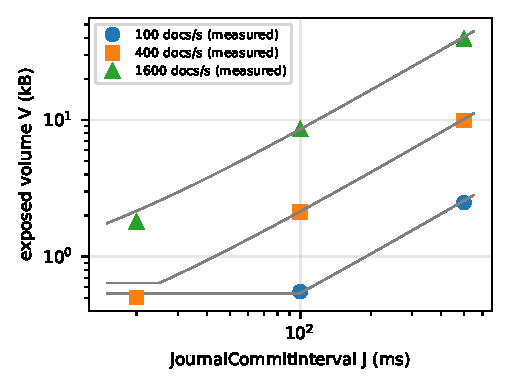
\includegraphics[width=\columnwidth]{figures/fig_plant.pdf}
\caption{Static plant: measured exposed volume versus $J$ at three loads, with the model (grey).}\label{fig:plant}
\end{figure}
\begin{table}[t]\centering\small
\caption{Static plant: measured exposed volume $V$ (kB per sync) versus the model $V=R(J+pL_0)/p$, $p=\min(1,RJ/b_0)$, $b_0=513$\,B, $L_0=7$\,ms.}\label{tab:plant}
\resizebox{\columnwidth}{!}{\begin{tabular}{rrrrrr}\toprule
Load (docs/s) & $J$ (ms) & $R$ (kB/s) & $V$ meas. & $V$ model & err. (\%)\\\midrule
100 & 500 & 5.1 & 2.49 & 2.57 & +3.4\\
100 & 100 & 5.1 & 0.56 & 0.54 & -2.3\\
100 & 20 & 5.0 & 0.50 & 0.54 & +6.9\\
400 & 500 & 20.0 & 9.92 & 10.16 & +2.4\\
400 & 100 & 20.0 & 2.13 & 2.14 & +0.7\\
400 & 20 & 20.0 & 0.50 & 0.64 & +27.8\\
1600 & 500 & 80.1 & 39.24 & 40.60 & +3.5\\
1600 & 100 & 80.0 & 8.58 & 8.57 & -0.1\\
1600 & 20 & 80.0 & 1.79 & 2.16 & +20.9\\
\bottomrule\end{tabular}}\end{table}


\textbf{Dynamics and noise.} A load step from 400 to 1600 documents/s with $J$ fixed multiplied $V$ by 4.05 (load ratio 3.98). The 10\,s window makes the sensor the dominant dynamics: $V$ reaches 63\,\% of its final value after 6.5--7\,s and 95\,\% after 10\,s, whereas the per-tick byte rate $\hat R$ reaches 90\,\% after 2\,s. The actuator takes 4.9\,ms on average, far below the 0.5\,s period. The noise of $V$ is mainly counting: at $J=500$\,ms a window holds about 20 syncs, so one sync changes $V$ by 5\,\%, and the relative standard deviation is \vcvMinHundred--\vcvMaxHundred\,\% at 100\,ms. The per-tick byte rate is close to white (relative sd \rcvBaseMin--\rcvBaseMax\,\% at 400 documents/s). The closed-loop floor of 1.2--1.5\,\% is of the same order (Table~\ref{tab:noise}).
\begin{table}[t]\centering\small
\caption{Measurement noise of the 10\,s signal $V$ (relative standard deviation over a 60\,s segment, open loop) and syncs per window.}\label{tab:noise}
\begin{tabular}{rrrr}\toprule
Load (docs/s) & $J$ (ms) & $\mathrm{sd}(V)/V$ (\%) & syncs per 10\,s\\\midrule
100 & 500 & 5.4 & 20\\
100 & 100 & 4.1 & 91\\
100 & 20 & 0.6 & 101\\
400 & 500 & 5.8 & 20\\
400 & 100 & 1.1 & 94\\
400 & 20 & 0.3 & 399\\
1600 & 500 & 5.8 & 20\\
1600 & 100 & 1.3 & 93\\
1600 & 20 & 0.4 & 448\\
\bottomrule\end{tabular}\end{table}


\section{Controllers and Tuning}\label{sec:controllers}
All controllers work on $e=\ln V^*-\ln\hat V$ and command $J\in[20,500]$\,ms every 0.5\,s; $V^*=4096$\,B (Fig.~\ref{fig:scheme}).
\begin{figure}[t]\centering
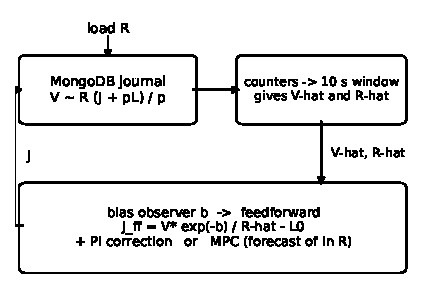
\includegraphics[width=\columnwidth]{figures/fig_scheme.pdf}
\caption{Control structure shared by all controllers. FF+obs has no PI/MPC block; PI has no feedforward; the MPC replaces the PI correction by an optimisation over a forecast of the load.}\label{fig:scheme}
\end{figure}

\textbf{PI.} $u=\ln J=u_0+K_pe+K_i\sigma$ with $\sigma\leftarrow\sigma+\Delta t\,e$, clamp or back-calculation anti-windup, and optional filtering of $\ln\hat V$. It acts on the windowed signal; the load-aware controllers also use $\hat R$.

\textbf{Feedforward with observer (FF+obs).} $J_{\rm ff}=V^*e^{-b}/\hat R-L_0$, where the bias $b$ is an exponential average of $\ln V_{\rm measured}-\ln V_{\rm model}$ over the same window; it absorbs model error and compensates the sensor lag. No feedback gain, no prediction. \textbf{PI-FF} adds the PI correction to the same feedforward.

\textbf{PI on a fast estimate (PI-fast).} A PI on $\ln\hat V_{\rm fast}=\ln v(\hat R,J_{k-1})+b$, the static law $v$ evaluated at the current load estimate and the last applied interval, corrected by the same observer. It separates the value of a fast signal from that of the structure: no feedforward term, no prediction.

\textbf{MPC.} At each tick, $u=\ln J$ minimises $\sum_{i=1}^{H}\gamma^{i-1}s(e_i)e_i^2+\lambda(u-u_{\rm prev})^2$ with $e_i=\ln V^*-[\ln v(\hat R_{k+i},e^{u})+b]$ and $s=w$ below the target, 1 otherwise. $\hat R_{k+i}$ is forecast by persistence, moving average (level plus slope) or ARIMA(1,1,0) on a 5-sample window: light forecasters. The scalar problem is solved by grid search with golden-section refinement. With $H=1$ and $\lambda\to0$ the MPC reduces to FF+obs (checked numerically); with $\lambda>0$ it acts as FF+obs followed by smoothing of the command.

\textbf{Operator baselines.} \emph{Static} keeps the engine default $J=100$\,ms. \emph{Threshold} is a rule-based manager: on the windowed $V$, if $V/V^*>h$ it multiplies $J$ by $d<1$, if $V/V^*<l$ by $u>1$, otherwise it holds, at most once every $c$ ticks, $J$ bounded.

\textbf{Tuning.} Each family received the same budget of 60 random candidates on a calibrated simulator, with a robust objective (half nominal plant, half stress plant with slower sync, more jitter and one tick of delay) and tuning seeds disjoint from test seeds; families added by amendments (PI-fast, Threshold, and each new cell) were tuned the same way. The three MPC predictors share candidates. Search ranges were widened once after a first run placed continuous optima on an edge; the remaining edge values are the ``no filtering'' options and extremes of discrete sets. A first tuning gave the MPC an apparent advantage traced to a different smoothing of the load estimate; all controllers now receive raw inputs and tune their own. PI-fast: $K_p=2.75$, $K_i=0.98$; Threshold: $h=1.44$, $l=0.93$, $d=0.18$, $u=1.41$, $c=16$ ticks on the step. All specifications are in the repository; Table~\ref{tab:params} lists the parameters of the main study.
\begin{table*}[t]\centering\small
\caption{Controller parameters used in all runs (random search, 60 candidates per family, robust objective; nominal values from the repository file \texttt{tuned\_specs.json}). PI-default is the naive reference (no tuning). Dashes: parameter not used by the family.}\label{tab:params}
\resizebox{\textwidth}{!}{\begin{tabular}{lccccccccccc}\toprule
Controller & $K_p$ & $K_i$ & anti-windup & $\alpha_V$ & feedforward & $\alpha_{R}$ & bias $\alpha_b$ & $H$ & $\gamma$ & $\lambda$ & $w$ (below target)\\\midrule
PI-default & 0.3 & 0.05 & clamp & 1 & no & -- & -- & -- & -- & -- & --\\
PI (tuned) & 3.19 & 0.35 & backcalc & 1 & no & -- & -- & -- & -- & -- & --\\
PI-FF & 3.66 & 0.19 & backcalc & 1 & yes & 1 & 0 & -- & -- & -- & --\\
PI-fast & 2.75 & 0.98 & backcalc & 0.25 & no (fast $\hat V$) & 0.6 & 0.6 & -- & -- & -- & --\\
FF+obs & 0.00 & 0.00 & clamp & 1 & yes & 1 & 1 & -- & -- & -- & --\\
MPC persistence & -- & -- & -- & -- & -- & 1 & 1 & 10 & 0.85 & 0.020 & 0.62\\
MPC moving average & -- & -- & -- & -- & -- & 0.3 & 1 & 3 & 0.7 & 0.024 & 0.86\\
MPC ARIMA(1,1,0) & -- & -- & -- & -- & -- & 0.3 & 1 & 3 & 0.7 & 0.024 & 0.86\\
\bottomrule\end{tabular}}
\\[2pt]{\footnotesize Common: $V^*=4096$\,B, period 0.5\,s, $J\in[20,500]$\,ms, $J_0=100$\,ms, window 10\,s, $b_0=513$\,B, $L_0=7$\,ms; MA/ARIMA window 5 / 5 samples (persistence ignores it). $\alpha_V$: filter on $\ln V$; $\alpha_R$: smoothing of the load estimate; $\alpha_b$: bias observer.}\end{table*}


\section{Experimental Protocol}\label{sec:protocol}
\textbf{Platform and workload.} A Kind cluster (Kubernetes v1.27.3, one control plane, three workers) on a single Windows host under WSL2 (6\,GB), MongoDB 8.0.32 in one authenticated pod. The generator inserts batches of 10 documents with four threads at a regulated rate, write concern $w=1$, $j=$false, so the exposure window is set by $J$.

\textbf{Scenarios.} Stationary (400 documents/s); step burst (400$\to$1600 documents/s from $t=100$ to 160\,s); low load (100$\to$400 documents/s, target unreachable, actuator saturates). Runs last 300\,s with a 20\,s warm-up. Amendment 5 adds a triangular ramp (400$\to$1600$\to$400 documents/s over 120\,s), a periodic load (raised cosine, period 40\,s, three periods) and a 1\,s actuation delay injected by the runner: the command computed at tick $k$ is applied two ticks later and the controller is not told, as for an operator acting through an API.

\textbf{Design.} Controllers run in randomised, interleaved blocks, 30\,s apart. A run is invalid and repeated if a pod restarts, the acknowledged rate falls below 95\,\% of the offered rate, or insertions fail. A pilot of 63 runs (3 per cell) preceded a campaign of 71 runs with the same specifications, pooled; cell sizes were set from the pilot and are unequal (Table~\ref{tab:main}). No batch effect is detected on the burst error or the peak (pilot against campaign, exact Mann--Whitney $p>0.1$, low power).

\textbf{Amendments, written and committed before each block's first run.} (4) A block of 30 runs of the burst scenario (PI-fast, PI, FF+obs, 10 each), analysed alone with contemporaneous controls; three readings were fixed in advance (PI-fast equivalent to FF+obs, in between, or equivalent to PI). (5) Three cells (ramp; periodic; periodic with delay) $\times$ four controllers (PI, FF+obs, MPC persistence, MPC ARIMA) $\times$ 8 runs, one interleaved plan of 96 runs, each family re-tuned per cell, Holm correction over 18 declared contrasts. (6) Block A repeats the single suggestive contrast of amendment 5 (ARIMA against FF+obs, periodic, no delay) on 12 new runs per controller with one declared test (two-sided Mann--Whitney, $\alpha=0.05$, no correction, confirmed if $p<0.05$ and ARIMA is lower); block B compares Static and Threshold with a contemporaneous FF+obs on the step and the periodic load (8 runs each, Holm over 8 tests). All blocks were fully valid.

\textbf{Analysis.} Errors are $|V/V^*-1|$. Primary criteria on the burst: the mean error from the start of the burst to 20\,s after its end (burst error) and the exposure peak (maximum of $V$ over 4\,s windows relative to $V^*$). Seven contrasts in the main study, Mann--Whitney tests with Holm correction over 14 tests, Cliff's $\delta$ and bootstrap CIs; equivalence (TOST on the Welch 90\,\% CI) where the claim is ``no difference'', with margins of 0.7 percentage points (burst error) and 0.10 (peak), about half the steady-state noise floor.

\section{Results}\label{sec:results}
\textbf{Summary of findings.} Fig.~\ref{fig:summary} shows the burst error of every controller in every cell. RQ1: knowing the load is what matters (PI \MaePITS\,\% against \MaePIFFS--\MaeMPCMS\,\% on the step), a PI on a fast estimate recovers about 60\,\% of the gap, and the structure explains the rest. RQ2: forecasting brings nothing on steps and ramps and about 0.4 pp (18\,\%) with ARIMA on a periodic load; with a 1\,s delay no significant gain. RQ3: the engine default and tuned threshold rules have 18--89\,\% error, one to two orders of magnitude above the feedforward.
\begin{figure*}[t]\centering
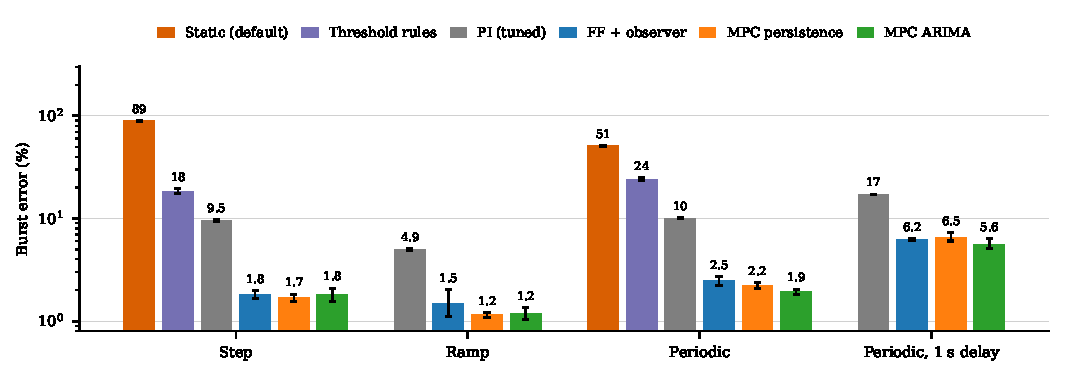
\includegraphics[width=0.95\textwidth]{figures/fig_summary.pdf}
\caption{Burst error (mean and 95\,\% bootstrap CI, log scale) of every controller in every cell. Step: main study (PI $n=6$; FF+obs and MPC persistence $n=15$; ARIMA $n=10$; one stalled run excluded) and amendment 6 baselines ($n=8$); other cells: amendments 5 and 6 ($n=8$).}\label{fig:summary}
\end{figure*}

\textbf{Data.} 135 main runs, 30 PI-fast runs, 96 runs of amendment 5, 72 of amendment 6 and 81 sensitivity runs, all valid; no pod restarted during any run, acknowledged/offered rate between 0.964 and 1.002.

\textbf{Step burst.} Table~\ref{tab:main} and Figs.~\ref{fig:burst} and~\ref{fig:primary} summarise the main study. The tuned PI has a burst error of \MaePITS\,\% (sd \MaeSdPITS) and a peak of \PeakPITS$\times V^*$, against \MaePIFFS\,\% (PI-FF), \MaeFFOS\,\% (FF+obs) and \MaeMPCPS\,\% (MPC persistence), with peaks of \PeakPIFFS, \PeakFFOS\ and \PeakMPCPS. The PI-versus-PI-FF difference is $+$\cDMaePITPIFFS\ pp (95\,\% CI [\cLoMaePITPIFFS, \cHiMaePITPIFFS], $p_{\rm Holm}=\cPHMaePITPIFFS$). FF+obs versus MPC persistence is $+$\cDMaeFFOMPCPS\ pp [\cLoMaeFFOMPCPS, \cHiMaeFFOMPCPS] on the burst error and \cDPeakFFOMPCPS\ on the peak; the equivalence tests conclude equivalence on both criteria once one stalled run is set aside (see below) and are inconclusive with it, while the rank tests do not change. MPC with a moving average is worse than persistence by \cAMaeMPCPMPCMS\ pp and ARIMA is equivalent to it: neither forecaster improves on persistence. PI-FF has the lowest burst error on the main platform, \cAMaePIFFMPCPS\ pp below MPC, with no difference on the peak; this did not replicate on the second platform. It also moves $J$ about twice as much as MPC and recovers more slowly when the actuator saturates (low-load scenario).
\begin{table}[t]\centering\footnotesize
\caption{Step burst (400$\to$1600 documents/s for 60\,s), mean (sd) over $n$ valid runs (pilot included; the one run with a journal-sync stall of 5\,s or more is excluded here). Peak: maximum of $V$ over 4\,s windows, relative to $V^*$.}\label{tab:main}
\begin{tabular}{lrccc}\toprule
Controller & $n$ & Burst error (\%) & Peak ($\times V^*$) & $|\Delta\ln J|$\\\midrule
PI (default gains) & 3 & 55.51 (1.80) & 2.71 (0.03) & 0.005\\
PI (tuned) & 6 & 9.55 (0.15) & 1.88 (0.09) & 0.043\\
PI + feedforward & 15 & 1.25 (0.17) & 1.36 (0.05) & 0.055\\
FF + observer & 15 & 1.82 (0.30) & 1.34 (0.07) & 0.032\\
MPC, persistence & 15 & 1.69 (0.28) & 1.36 (0.04) & 0.026\\
MPC, moving average & 10 & 2.81 (0.45) & 1.50 (0.08) & 0.024\\
MPC, ARIMA(1,1,0) & 10 & 1.83 (0.46) & 1.40 (0.14) & 0.028\\
\bottomrule\end{tabular}\end{table}

\begin{figure*}[t]\centering
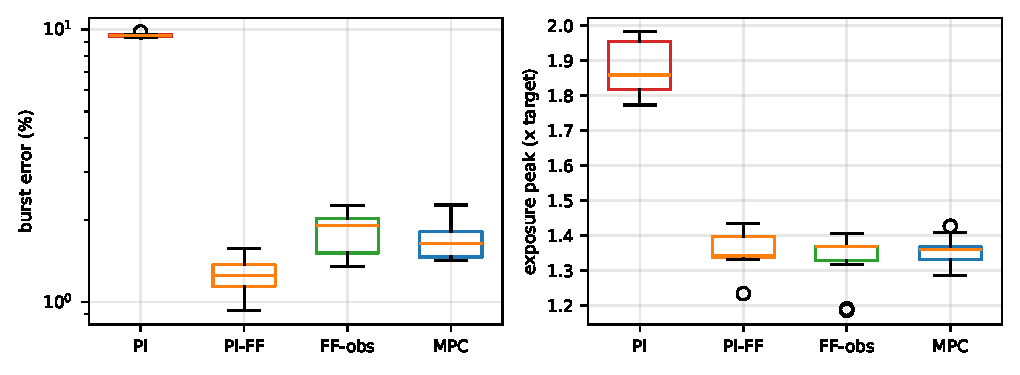
\includegraphics[width=0.7\textwidth]{figures/fig_primary.pdf}
\caption{Step burst: primary criteria per controller (boxes: quartiles; points: outliers).}\label{fig:primary}
\end{figure*}
Table~\ref{tab:contrasts} gives the seven declared contrasts with Holm correction and Table~\ref{tab:equiv} the equivalence tests.
\begin{table*}[t]\centering\small
\caption{Pre-specified contrasts (Mann--Whitney U, two-sided; Holm correction over the 14 tests = 7 contrasts $\times$ 2 primary criteria). Difference = mean(A) $-$ mean(B) with 95\% bootstrap CI; $\delta$ = Cliff's delta. ``All runs'' includes the stalled run; ``excl.'' removes it (post hoc sensitivity analysis).}\label{tab:contrasts}
\resizebox{\textwidth}{!}{\begin{tabular}{llccccc}\toprule
 & Contrast (A vs B) & Difference [95\% CI] (all runs) & $\delta$ & $p_{\text{Holm}}$ (all) & Difference [CI] (excl.) & $p_{\text{Holm}}$ (excl.)\\\midrule
\multicolumn{7}{l}{\emph{Burst error (pp)}}\\
 & PI vs PI-FF & +8.30 [+8.17, +8.44] & +1.00 & $4.4\!\times\!10^{-4}$ & +8.30 [+8.17, +8.44] & $4.4\!\times\!10^{-4}$\\
 & PI-FF vs FF+obs & -11.17 [-32.44, -0.44] & -0.93 & $1.8\!\times\!10^{-4}$ & -0.57 [-0.74, -0.40] & $2.7\!\times\!10^{-4}$\\
 & FF+obs vs MPC-pers. & +10.73 [-0.02, +32.03] & +0.35 & $0.605$ & +0.13 [-0.07, +0.32] & $0.951$\\
 & PI-FF vs MPC-pers. & -0.44 [-0.61, -0.29] & -0.92 & $2.5\!\times\!10^{-4}$ & -0.44 [-0.61, -0.29] & $2.7\!\times\!10^{-4}$\\
 & MPC-pers. vs MPC-MA & -1.12 [-1.42, -0.83] & -0.95 & $9.2\!\times\!10^{-4}$ & -1.12 [-1.42, -0.83] & $9.2\!\times\!10^{-4}$\\
 & MPC-pers. vs MPC-ARIMA & -0.14 [-0.43, +0.17] & -0.15 & $1.000$ & -0.14 [-0.43, +0.17] & $1.000$\\
 & PI vs MPC-pers. & +7.86 [+7.68, +8.03] & +1.00 & $4.4\!\times\!10^{-4}$ & +7.86 [+7.68, +8.03] & $4.4\!\times\!10^{-4}$\\
\multicolumn{7}{l}{\emph{Peak ($\times V^*$)}}\\
 & PI vs PI-FF & +0.52 [+0.45, +0.59] & +1.00 & $0.005$ & +0.52 [+0.45, +0.59] & $0.005$\\
 & PI-FF vs FF+obs & -2.33 [-7.07, +0.05] & +0.10 & $1.000$ & +0.02 [-0.01, +0.06] & $1.000$\\
 & FF+obs vs MPC-pers. & +2.34 [-0.05, +7.07] & +0.06 & $1.000$ & -0.02 [-0.06, +0.01] & $1.000$\\
 & PI-FF vs MPC-pers. & +0.00 [-0.03, +0.03] & +0.09 & $1.000$ & +0.00 [-0.03, +0.03] & $1.000$\\
 & MPC-pers. vs MPC-MA & -0.15 [-0.20, -0.09] & -0.81 & $0.005$ & -0.15 [-0.20, -0.09] & $0.005$\\
 & MPC-pers. vs MPC-ARIMA & -0.04 [-0.13, +0.04] & -0.25 & $1.000$ & -0.04 [-0.13, +0.04] & $1.000$\\
 & PI vs MPC-pers. & +0.52 [+0.46, +0.59] & +1.00 & $0.005$ & +0.52 [+0.46, +0.59] & $0.005$\\
\bottomrule\end{tabular}}\end{table*}

\begin{table}[t]\centering\small
\caption{Equivalence tests (TOST, Welch 90\% CI inside $\pm$ margin; margins 0.7\,pp on the burst error and 0.10 on the peak).}\label{tab:equiv}
\resizebox{\columnwidth}{!}{\begin{tabular}{lccc}\toprule
Pair, criterion & 90\% CI (excl.) & verdict (excl.) & verdict (all)\\\midrule
FF+obs vs MPC-pers., error & [-0.05, +0.31] & equivalent & inconclusive\\
MPC-pers. vs MPC-ARIMA, error & [-0.42, +0.15] & equivalent & equivalent\\
FF+obs vs MPC-pers., peak & [-0.05, +0.01] & equivalent & inconclusive\\
MPC-pers. vs MPC-ARIMA, peak & [-0.12, +0.04] & inconclusive & inconclusive\\
\bottomrule\end{tabular}}\end{table}

\begin{figure}[t]\centering
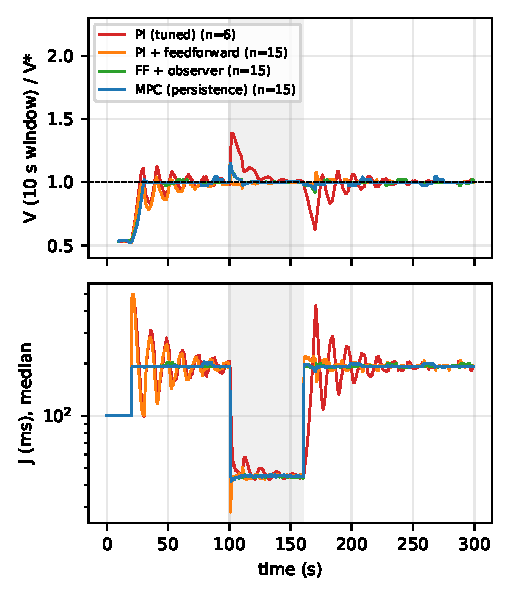
\includegraphics[width=\columnwidth]{figures/fig_burst.pdf}
\caption{Step burst, median over valid runs, stalled run excluded (shaded: burst). Top: $V$ over a 10\,s window relative to the target. Bottom: commanded $J$.}\label{fig:burst}
\end{figure}

The stationary and low-load scenarios (Table~\ref{tab:other}) are descriptive.
\begin{table}[t]\centering\small
\caption{Stationary (400 documents/s) and low-load (100$\to$400 documents/s, target unreachable at the start) scenarios, mean over $n_{\rm st}$ stationary runs and $n_{\rm ll}$ low-load runs (stationary runs: pilot only, descriptive).}\label{tab:other}
\resizebox{\columnwidth}{!}{\begin{tabular}{lccccc}\toprule
Controller & Stat. err. (\%) & Low-load err. (\%) & Recov. (s) & $n_{\rm st}$ & $n_{\rm ll}$\\\midrule
PI-def. & 26.08 & 49.83 & -- & 3 & 3\\
PI & 1.32 & 28.78 & 1.8 & 3 & 6\\
PI-FF & 1.38 & 31.48 & 24.1 & 3 & 6\\
FF+obs & 1.34 & 28.18 & 2.9 & 3 & 6\\
MPC-pers. & 1.22 & 28.01 & 3.0 & 3 & 6\\
MPC-MA & 1.31 & 28.22 & 2.3 & 3 & 6\\
MPC-ARIMA & 1.49 & 28.27 & 2.8 & 3 & 6\\
\bottomrule\end{tabular}}\end{table}


\textbf{Simulator versus real cluster.} The simulator was calibrated on the static grid (worst error 3.9\,\% on $V$) and on the burst response. On the pilot the ranking of the seven controllers by burst error is identical to the simulated one (Spearman 1.00), with real-to-simulated ratios between 0.80 and 1.09; but the simulator underestimates the steady-state noise (real error 1.2--1.5\,\% against 0.5--0.95\,\%) and the between-run variability, so it was used for tuning and design only.

\textbf{A journal-sync stall.} One FF+obs run (the first after the pod was recreated) shows no journal sync for 12.5\,s during the burst; its burst error is 171\,\% and its peak $39\times V^*$. It is valid under the pre-specified rules and included in the primary analysis; a sensitivity analysis excludes runs with a sync gap of 5\,s or more (post hoc, defined from the counters). The cause is unknown.

\textbf{PI on a fast estimate (amendment 4).} All 30 runs were valid (Table~\ref{tab:pifast}). PI-fast has a burst error of 5.01\,\% (sd 0.75), between the PI (9.62\,\%) and FF+obs (1.93\,\%) of the same block; these controls agree with the main study (9.55\,\% and 1.82\,\%). The four declared contrasts are significant after Holm correction ($p_{\rm H}=0.0007$, Cliff's $\delta=\pm1$): PI-fast minus PI is $-4.61$ pp (CI [$-5.00$, $-4.09$]) on the error and $-0.25$ on the peak; PI-fast minus FF+obs is $+3.09$ pp ([2.62, 3.62]) and $+0.21$. No equivalence was concluded, and the distributions do not overlap. PI-fast closes 60\,\% of the burst-error gap between PI and FF+obs (CI 53--66\,\%) and 55\,\% of the peak gap: the second pre-specified reading. Unexpectedly, the PI-fast error increases with run order (Spearman 0.82, $p=0.004$; 4.45--4.70\,\% in the first five runs, 4.75--6.90\,\% in the last five), with no significant trend for PI or FF+obs; the cause is not investigated, and the ordering of the three controllers does not depend on it.
\begin{table}[t]\centering\footnotesize
\caption{PI-fast block (amendment 4): burst scenario, mean (sd) over 10 valid runs per controller, run contemporaneously and analysed alone. Last row: share of the PI-to-FF+obs difference closed by PI-fast (95\,\% bootstrap CI).}\label{tab:pifast}
\begin{tabular}{lccc}\toprule
Controller & Burst error (\%) & Peak ($\times V^*$) & Recovery (s)\\\midrule
PI (tuned) & 9.62 (0.22) & 1.87 (0.07) & 11.0\\
PI-fast & 5.01 (0.75) & 1.62 (0.04) & 8.8\\
FF + observer & 1.93 (0.43) & 1.41 (0.04) & 2.0\\\midrule
Gap closed & 60\,\% [53, 66] & 55\,\% [44, 67] & --\\
\bottomrule\end{tabular}\end{table}


\textbf{Other disturbances and delay (amendment 5).} In none of the 18 declared tests does a predictor beat FF+obs after Holm correction (Table~\ref{tab:scn}). On the ramp, MPC persistence (1.16\,\%) and FF+obs (1.49\,\%) cannot be told apart (difference 0.33 pp, CI [$-0.04$, 0.88]); FF+obs has a larger spread there because of one slow run. On the periodic load, MPC with ARIMA has the lowest error (1.95\,\% against 2.47\,\%; difference 0.53 pp, CI [0.26, 0.79], unadjusted $p=0.005$, $p_{\rm H}=0.084$): suggestive, not significant under the declared correction. With the 1\,s delay every controller degrades and the PI collapses (17.2\,\%, no recovery in the window); ARIMA is on average lower than FF+obs (5.64\,\%, $p_{\rm H}=0.17$) but with a spread six times larger and a higher peak (1.41 against $1.31\times V^*$). No trend with run order appears.
\begin{table}[t]\centering\footnotesize
\caption{Amendment 5: mean (sd) over 8 valid runs per cell and controller; each family re-tuned per cell. $p_{\rm H}$: Mann--Whitney $p$ against FF+obs on the error, Holm-corrected over the 18 declared tests.}\label{tab:scn}
\begin{tabular}{llccc}\toprule
Cell & Controller & Error (\%) & Peak & $p_{\rm H}$\\\midrule
Ramp & PI & 4.93 (0.21) & 1.20 (0.10) & --\\
 & FF+obs & 1.49 (0.73) & 1.13 (0.15) & --\\
 & MPC pers. & 1.16 (0.10) & 1.07 (0.02) & 1\\
 & MPC ARIMA & 1.20 (0.23) & 1.08 (0.02) & 1\\\midrule
Periodic & PI & 10.06 (0.11) & 1.30 (0.04) & --\\
 & FF+obs & 2.47 (0.36) & 1.15 (0.04) & --\\
 & MPC pers. & 2.21 (0.22) & 1.13 (0.03) & 1\\
 & MPC ARIMA & 1.95 (0.18) & 1.12 (0.04) & 0.084\\\midrule
Periodic, & PI & 17.17 (0.17) & 1.67 (0.05) & --\\
1\,s delay & FF+obs & 6.25 (0.16) & 1.31 (0.03) & --\\
 & MPC pers. & 6.48 (1.05) & 1.35 (0.17) & 1\\
 & MPC ARIMA & 5.64 (1.01) & 1.41 (0.27) & 0.17\\
\bottomrule\end{tabular}\end{table}


\textbf{Confirmation and operator baselines (amendment 6).} The declared test of block A is confirmed on the new runs (Table~\ref{tab:amend6}): on the periodic load MPC with ARIMA has a burst error of 1.85\,\% (sd 0.28) against 2.26\,\% (0.15) for FF+obs, $-0.40$ pp (CI [$-0.56$, $-0.21$], Cliff's $\delta=-0.83$, $p=0.0006$), with the same peak and the same I/O cost; the gain is about 18\,\% of the error. In block B the baselines are far from the load-aware controller: the engine default has a burst error of 89.4\,\% on the step and 50.9\,\% on the periodic load, with an exposure peak of $2.2\times V^*$; threshold rules, tuned per cell, reduce it to 18.3\,\% and 24.1\,\% (peak 2.16 and $2.05\times V^*$), and some runs do not recover inside the run; FF+obs has 1.76\,\% and 2.52\,\%. None of the baselines saves synchronisation work (9.4 and 8.5--10.0 syncs/s against 8.6).
\begin{table}[t]\centering\footnotesize
\caption{Amendment 6. Top: confirmation on the periodic load, 12 new runs per controller. Bottom: operator baselines against a contemporaneous FF+obs, 8 runs per cell and controller. Static: $J=100$\,ms never changed; Threshold: rule-based manager. All eight contrasts against FF+obs: Holm $p_{\rm H}\le0.0036$.}\label{tab:amend6}
\begin{tabular}{llccc}\toprule
Block & Controller & Error (\%) & Peak & Syncs/s\\\midrule
Confirm., & FF+obs & 2.26 (0.15) & 1.13 (0.02) & 8.63\\
periodic & MPC ARIMA & 1.85 (0.28) & 1.13 (0.03) & 8.65\\\midrule
Step & Static & 89.38 (1.72) & 2.24 (0.04) & 9.39\\
 & Threshold & 18.28 (1.79) & 2.16 (0.05) & 8.51\\
 & FF+obs & 1.76 (0.30) & 1.35 (0.03) & 8.62\\\midrule
Periodic & Static & 50.89 (0.80) & 2.24 (0.12) & 9.39\\
 & Threshold & 24.09 (1.13) & 2.05 (0.07) & 10.00\\
 & FF+obs & 2.52 (0.33) & 1.20 (0.12) & 8.62\\
\bottomrule\end{tabular}\end{table}


\textbf{Sensitivity (descriptive, $n=3$ per variant).} Each continuous parameter of PI, PI-FF, FF+obs and MPC was perturbed by $\times0.5$ and $\times1.5$, and the target was changed. The worst ratio of burst error to the concurrent nominal is PI \SensWorstPIT, FF+obs \SensWorstFFO, MPC \SensWorstMPCP\ and PI-FF \SensWorstPIFF; for FF+obs and MPC the only large ratio comes from the smoothing of the load estimate (halving its factor multiplies the error by \SensSmoothFFO\ and \SensSmoothMPCP). PI-FF is the only controller with an unstable run: at $K_p\times1.5$ one of three runs oscillated (burst error 10.5\,\%, peak $20\times V^*$), coinciding with a journal-sync stall, so the gain and the stall cannot be separated. The ranking of load-aware controllers against the best PI variant survives on the burst error and not on the peak for PI-FF; we report the pre-specified criterion C2 as not satisfied on the peak. Journal syncs per second follow $1/V^*$ (about 17, 8.6 and 4.3 per second for $V^*=2048$, 4096 and 8192\,B); Tables~\ref{tab:sens} and~\ref{tab:vstar} give the details.
\begin{table}[t]\centering\small
\caption{Sensitivity to controller parameters (burst scenario, $n=3$ per variant, one-at-a-time, descriptive). Ratios are relative to 3 concurrent nominal runs of the same controller. Nominal: PI \MaeSensPITnom\,\%, PI-FF \MaeSensPIFFnom\,\%, FF+obs \MaeSensFFOnom\,\%, MPC \MaeSensMPCPnom\,\%.}\label{tab:sens}
\resizebox{\columnwidth}{!}{\begin{tabular}{llcccc}\toprule
Controller & Variant & Error (\%) & Ratio & Peak ($\times V^*$) & $|\Delta\ln J|$\\\midrule
PI & $K_i\times0.5$ & 14.79 & 1.58 & 1.82 & 0.041\\
PI & $K_i\times1.5$ & 8.07 & 0.86 & 2.08 & 0.048\\
PI & $K_p\times0.5$ & 11.35 & 1.21 & 2.16 & 0.024\\
PI & $K_p\times1.5$ & 8.52 & 0.91 & 1.77 & 0.063\\
PI-FF & $\alpha_R\times0.5$ & 2.44 & 2.16 & 1.47 & 0.048\\
PI-FF & $K_i\times0.5$ & 2.98 & 2.63 & 1.32 & 0.057\\
PI-FF & $K_i\times1.5$ & 1.33 & 1.18 & 1.42 & 0.059\\
PI-FF & $K_p\times0.5$ & 1.47 & 1.30 & 1.33 & 0.043\\
PI-FF & $K_p\times1.5$ & 4.76 & 4.20 & 7.45 & 0.094\\
FF+obs & $\alpha_b\times0.5$ & 1.68 & 1.02 & 1.41 & 0.029\\
FF+obs & $\alpha_R\times0.5$ & 3.18 & 1.93 & 1.54 & 0.016\\
MPC-pers. & $\alpha_b\times0.5$ & 1.43 & 0.90 & 1.36 & 0.020\\
MPC-pers. & $\alpha_R\times0.5$ & 3.70 & 2.32 & 1.61 & 0.023\\
MPC-pers. & $\lambda\times0.5$ & 1.85 & 1.16 & 1.37 & 0.032\\
MPC-pers. & $\lambda\times1.5$ & 1.49 & 0.93 & 1.33 & 0.023\\
MPC-pers. & $w\times0.5$ & 1.51 & 0.95 & 1.33 & 0.026\\
MPC-pers. & $w\times1.5$ & 1.47 & 0.92 & 1.42 & 0.023\\
\bottomrule\end{tabular}}\end{table}

\begin{table}[t]\centering\small
\caption{Change of the target $V^*$ (burst, $n=3$): error, peak and journal syncs per second. At $V^*=2048$\,B the target is unreachable during the burst ($J$ would be below 20\,ms).}\label{tab:vstar}
\begin{tabular}{llccc}\toprule
Controller & $V^*$ (B) & Error (\%) & Peak & syncs/s\\\midrule
PI-FF & 2048 & 2.33 & 1.34 & 17.02\\
PI-FF & 4096 & 1.13 & 1.40 & 8.68\\
PI-FF & 8192 & 2.32 & 1.47 & 4.41\\
FF+obs & 2048 & 1.74 & 1.32 & 17.23\\
FF+obs & 4096 & 1.64 & 1.39 & 8.62\\
FF+obs & 8192 & 2.83 & 1.40 & 4.31\\
MPC-pers. & 2048 & 4.90 & 1.57 & 16.76\\
MPC-pers. & 4096 & 1.60 & 1.37 & 8.61\\
MPC-pers. & 8192 & 3.68 & 1.39 & 4.28\\
\bottomrule\end{tabular}\end{table}


\textbf{Replication on a second platform.} The step burst was replayed for PI, PI-FF, FF+obs and MPC persistence, 6 runs each, on a shared Linux runner (\CICpu, 4 vCPU) with MongoDB in plain Docker, without re-tuning; MongoDB 8.x needed a community allocator workaround whose effect on the measurements is not verified. All \CIN\ runs were valid. The pre-specified R1 (PI error at least three times that of each load-aware controller) is \CIRone, R2 (FF+obs and MPC equivalent) is \CIRtwo\ and R3 (PI has the highest peak) is \CIRthree. One finding did not replicate: PI-FF had a lower burst error than MPC on the main platform but the difference is \CIPIFFvsMPCD\ pp on the second platform (CI [\CIPIFFvsMPCLo, \CIPIFFvsMPCHi]), the opposite sign: it is platform-dependent (Table~\ref{tab:ci}).
\begin{table}[t]\centering\small
\caption{Replication on a second platform (shared Linux runner, MongoDB in plain Docker), burst scenario, mean (sd) over 6 runs; last column: same controller on the main platform.}\label{tab:ci}
\resizebox{\columnwidth}{!}{\begin{tabular}{lccccc}\toprule
Controller & Error (\%) & Peak ($\times V^*$) & $|\Delta\ln J|$ & syncs/s & Main platform (\%)\\\midrule
PI (tuned) & 9.36 (0.27) & 1.86 (0.11) & 0.044 & 8.54 & 9.55\\
PI + feedforward & 1.52 (0.06) & 1.38 (0.06) & 0.046 & 8.70 & 1.25\\
FF + observer & 1.45 (0.32) & 1.37 (0.03) & 0.022 & 8.63 & 1.82\\
MPC, persistence & 1.33 (0.12) & 1.37 (0.03) & 0.019 & 8.63 & 1.69\\
\bottomrule\end{tabular}}\end{table}


\section{Discussion}\label{sec:discussion}
\textbf{Why prediction does not help here.} The actuator acts on $V$ within one tick while the sensor is delayed by the 10\,s window, so a controller that knows $\hat R$ and the static law sets $J$ almost exactly; what remains is the sensor lag and model error, which the bias observer corrects. Forecasting $R$ several ticks ahead adds noise, not information, because the plant has no delay to compensate; the moving-average variant is worse, although it was also tuned with a smoother load estimate ($\alpha_R=0.3$ against 1), which alone roughly doubles the burst error of the persistence MPC when halved (Table~\ref{tab:sens}), so the effect of its slope term is not isolated. A step cannot be anticipated by any forecaster, so we tested a ramp, a periodic load and a 1\,s delay. Forecasting helps a little on the periodic load: ARIMA lowers the burst error by 0.4 pp (about 18\,\%), confirmed on new runs. That is the case a forecaster is built for, and the gain is small; persistence does not help, the ramp shows no gain, and with a delay the gain is not significant while the spread of the MPC is six times larger. We found no need for forecasting on steps and ramps, and a small gain on a deterministic periodic load.

\textbf{Why feedback alone fails.} Feedback on the windowed $V$ reacts only as the window fills: even tuned ($K_p=3.2$, $K_i=0.35$) the PI has a burst error five to eight times larger than the load-aware controllers and a peak 1.4 times higher. The PI-fast block separates signal speed from structure: a PI on a fast model-based estimate recovers about 60\,\% of the gap, so most of the benefit of the load-aware designs is the speed of the signal and the rest, a plausible reason being untested, comes from acting on the load directly rather than through an error. A Smith predictor and a PI on a purely measured short-window $V$ were not tested.

\textbf{Against operator practice.} The comparison that matters to an operator is not MPC against feedforward. The engine default leaves the exposure at $2.2\times V^*$ during a burst and tuned threshold rules keep 18--24\,\% error, against under 3\,\% for a load feedforward with an observer, at the same or lower I/O cost. A load-aware control is worth roughly an order of magnitude in exposure error here; which load-aware design is used is a second-order choice.

\textbf{What matters.} The controller structure matters less than the responsiveness of the load estimate: smoothing it more than the plant requires doubles the burst error for every load-aware controller (Table~\ref{tab:sens}), while the MPC weights and the observer factor are second order and, for PI-FF, the integral gain matters as much.

\textbf{Practical guidance.} On this engine and knob, a load feedforward with a model-bias observer is the simplest controller that attains the accuracy of MPC. The responsiveness of the load estimate matters more than the controller structure: smoothing it more than the plant requires doubles the burst error of every load-aware controller. With a 1\,s actuation delay the feedforward degrades gracefully (6.3\,\% error, sd 0.16 pp) where the PI collapses (17.2\,\%). Feedback is optional and should be added only with a measured gain margin.

\textbf{Which controller for which situation.} Table~\ref{tab:guide} turns the results into guidance; it applies to this engine, this knob and the profiles tested.
\begin{table*}[t]\centering\footnotesize
\caption{Guidance drawn from the measurements (burst error unless stated; single engine, profiles tested).}\label{tab:guide}
\begin{tabular}{p{0.24\textwidth}p{0.3\textwidth}p{0.38\textwidth}}\toprule
Situation & Choice & Evidence\\\midrule
Step or ramp load, fast actuator & Load feedforward with observer; MPC persistence is equivalent & 1.8\,\% and 1.7\,\% (step); ramp 1.5\,\% and 1.2\,\%, not distinguishable\\
Periodic load of known period, fast actuator & MPC with ARIMA if the gain justifies the complexity; otherwise feedforward & ARIMA 1.85\,\% against 2.26\,\% (confirmed on 12 new runs), same peak and I/O cost\\
Actuation delay of about 1\,s & Load feedforward; avoid feedback-only control & FF+obs 6.3\,\% (sd 0.16 pp); PI 17.2\,\%; ARIMA lower on average but six times more spread, not significant\\
No load signal, feedback only & Tuned PI on the fastest available estimate of $V$ & PI 9.6\,\%; PI on a fast estimate 5.0\,\%\\
Engine default or threshold rules & Replace by a load-aware controller & 89\,\% and 18\,\% (step), 51\,\% and 24\,\% (periodic), no saving in synchronisations\\
\bottomrule\end{tabular}\end{table*}

\textbf{Transferability.} The structure that makes feedforward sufficient here is generic to group-commit logging: the exposed data are proportional to the load times an interval set by the flush timer, and the actuator acts within a tick. Analogous knobs exist in other engines (for example \texttt{wal\_writer\_delay} and \texttt{commit\_delay} in PostgreSQL, \texttt{innodb\_flush\_log\_at\_timeout} in MySQL, the \texttt{appendfsync} policy in Redis), but we did not identify their plants, and whether the log-linear law and the conclusions carry over is a hypothesis, not a result.

\section{Limitations}\label{sec:limits}
(i) One engine, single-node deployments on two hosts; the second needed a community workaround for a MongoDB 8.x kernel incompatibility. (ii) $V$ is a composite of two counters and no crash-recovery experiment verifies it as data loss; no replication-level RPO is measured. (iii) The simulator underestimates noise and between-run variability; tuning was done on it and checked on a pilot. (iv) One run contains a journal-sync stall of unknown cause; one PI-FF run oscillated at a higher gain, coinciding with a stall. (v) Equivalence margins are set from the noise floor; the sensitivity analysis is descriptive ($n=3$) and one-at-a-time. (vi) One profile of each disturbance (step, ramp, 40\,s periodic load) and one delay (1\,s); the ARIMA gain was measured on a deterministic periodic profile, the most favourable case. (vii) PI-fast shares the static model with FF+obs, was tested in 10 runs per controller and drifts with run order for an unidentified reason; a PI on a purely measured short-window $V$ and a Smith predictor were not tested. (viii) The MPC is not delay-aware (it forecasts from the next tick, as a controller ignorant of the latency would); in simulation a delay-aware variant changes the periodic error by between $+2$ and $-3$\,\% for delays of 0.5 to 2\,s (10 seeds), which suggests the conclusion would not change, but this was not tested on the cluster. The moving-average and ARIMA forecasters are light and were tuned with a smoother load estimate than persistence, so the comparison does not isolate the forecaster. (ix) Cell sizes are unequal, the pilot is pooled with the campaign and the pod was recreated between them. (x) The baselines do not cover all operator practice (no proprietary autoscaler, no manual tuning); the threshold cooldown and, for MPC persistence, the horizon (20 ticks, the longest of the set) sit at the edge of the search sets. (xi) With 8 runs per cell the non-significant contrasts of amendment 5 should not be read as no effect; only the periodic ARIMA contrast was confirmed on new runs.

\section{Conclusion}\label{sec:conclusion}
On a real MongoDB deployment, using the observed write load is what lets a controller hold the exposed journal volume near its target during bursts, and about 60\,\% of the gain over a feedback-only PI is already obtained by feeding the PI a fast model-based estimate of that volume. Under a step burst, MPC with persistence forecasting is equivalent to a plain feedforward with a model-bias observer (once one stalled run is set aside). Forecasting helps only slightly and only on a periodic load, where ARIMA lowers the error by about 0.4 pp (18\,\%), confirmed on new runs; on a ramp and with a 1\,s actuation delay no gain was shown. Against operator practice the gain of any load-aware control is large: the engine default and tuned threshold rules have 18--89\,\% burst error against under 3\,\% for a feedforward. The ordering of PI against the load-aware controllers replicated on a second platform; the lower error of PI with feedforward did not. These conclusions are limited to the engine, the disturbance profiles and the platforms tested.

\section*{Acknowledgment}
An AI assistant (Claude, Anthropic) was used to support protocol design, to write and test the code of the controllers, the simulator, the run orchestration and the analysis scripts, to generate figures and tables, and to draft the text. All experiments were run by the authors on their own infrastructure, all reported data come from those runs, and every number in the tables and text is produced by the released scripts from the released run files. The authors reviewed and verified all outputs and take full responsibility for the content; the tool is not an author. No funding was received and the authors declare no competing interests. Run files, schedules, tuned specifications, amendments written before each data collection, code (\texttt{mpcrpo}), analysis scripts and the sources of this manuscript are available at \url{https://github.com/imanejerrari-etu-bit/mpc-rpo-mongodb}, release \texttt{v1.1}\repoRef. The full tables of the sensitivity analysis, the parameters of every controller and the extended text are in the supplementary file.

\begin{thebibliography}{99}
\bibitem{camacho2013model}
E.\ F.\ Camacho and C.\ Bordons.
\newblock \emph{Model Predictive Control}.
\newblock Advanced Textbooks in Control and Signal Processing.
  Springer-Verlag London, 2nd edition, 2007.

\bibitem{muske2002disturbance}
K.\ R.\ Muske and T.\ A.\ Badgwell.
\newblock Disturbance modeling for offset-free linear model predictive
  control.
\newblock \emph{Journal of Process Control}, 12(5):617--632, 2002.

\bibitem{pannocchia2003disturbance}
G.\ Pannocchia and J.\ B.\ Rawlings.
\newblock Disturbance models for offset-free model-predictive control.
\newblock \emph{AIChE Journal}, 49(2):426--437, 2003.

\bibitem{kothare1994antiwindup}
M.\ V.\ Kothare, P.\ J.\ Campo, M.\ Morari, and C.\ N.\ Nett.
\newblock A unified framework for the study of anti-windup designs.
\newblock \emph{Automatica}, 30(12):1869--1883, 1994.

\bibitem{astrom1989windup}
K.\ J.\ {\AA}str\"om and L.\ Rundqwist.
\newblock Integrator windup and how to avoid it.
\newblock In \emph{Proceedings of the 1989 American Control
  Conference}, pp.\ 1693--1698. IEEE, 1989.

\bibitem{roy2011autoscaling}
N.\ Roy, A.\ Dubey, and A.\ Gokhale.
\newblock Efficient autoscaling in the cloud using predictive models
  for workload forecasting.
\newblock In \emph{Proceedings of the IEEE 4th International
  Conference on Cloud Computing (CLOUD'11)}, pp.\ 500--507, 2011.

\bibitem{gong2010press}
Z.\ Gong, X.\ Gu, and J.\ Wilkes.
\newblock PRESS: PRedictive Elastic ReSource Scaling for cloud
  systems.
\newblock In \emph{Proceedings of the International Conference on
  Network and Service Management (CNSM)}, pp.\ 9--16, 2010.

\bibitem{cai2022inverse}
Z.\ Cai and R.\ Buyya.
\newblock Inverse queuing model-based feedback control for elastic
  container provisioning of web systems in Kubernetes.
\newblock \emph{IEEE Transactions on Computers}, 71(2):337--348, 2022.

\bibitem{pozdniakova2024sla}
O.\ Pozdniakova, D.\ Ma\v{z}eika, and A.\ Cholomskis.
\newblock SLA-adaptive threshold adjustment for a Kubernetes
  horizontal pod autoscaler.
\newblock \emph{Electronics}, 13(7):1242, 2024.

\bibitem{serracanta2025stability}
B.\ Serracanta, A.\ Luk\'acs, A.\ Rodriguez-Natal, A.\ Cabellos, and
  G.\ R\'etv\'ari.
\newblock On the stability of the Kubernetes horizontal autoscaler
  control loop.
\newblock \emph{IEEE Access}, 13:7160--7166, 2025.

\bibitem{baresi2016discrete}
L.\ Baresi, S.\ Guinea, A.\ Leva, and G.\ Quattrocchi.
\newblock A discrete-time feedback controller for containerized cloud
  applications.
\newblock In \emph{Proceedings of the 24th ACM SIGSOFT International
  Symposium on Foundations of Software Engineering (FSE 2016)}, pp.\
  217--228, 2016.

\bibitem{sabuhi2021adaptive}
M.\ Sabuhi, N.\ Mahmoudi, and H.\ Khazaei.
\newblock Optimizing the performance of containerized cloud software
  systems using adaptive PID controllers.
\newblock \emph{ACM Transactions on Autonomous and Adaptive Systems},
  15(3), 2021.

\bibitem{vanaken2017ottertune}
D.\ Van Aken, A.\ Pavlo, G.\ J.\ Gordon, and B.\ Zhang.
\newblock Automatic database management system tuning through
  large-scale machine learning.
\newblock In \emph{Proceedings of the 2017 ACM International
  Conference on Management of Data (SIGMOD'17)}, pp.\ 1009--1024, 2017.

\bibitem{zhang2019cdbtune}
J.\ Zhang, Y.\ Liu, K.\ Zhou, G.\ Li, Z.\ Xiao, B.\ Cheng, J.\ Xing,
  Y.\ Wang, T.\ Cheng, L.\ Liu, M.\ Ran, and Z.\ Li.
\newblock An end-to-end automatic cloud database tuning system using
  deep reinforcement learning.
\newblock In \emph{Proceedings of the 2019 ACM International
  Conference on Management of Data (SIGMOD'19)}, pp.\ 415--432, 2019.

\bibitem{ferreira2020selftunable}
L.\ Ferreira, F.\ Coelho, and J.\ Pereira.
\newblock Self-tunable DBMS replication with reinforcement learning.
\newblock In \emph{Distributed Applications and Interoperable Systems
  (DAIS 2020)}, LNCS vol.\ 12135, pp.\ 131--147. Springer, 2020.

\bibitem{joshi2024arimapid}
N.\ S.\ Joshi, R.\ Raghuwanshi, Y.\ M.\ Agarwal, B.\ Annappa, and
  D.\ N.\ Sachin.
\newblock ARIMA-PID: container auto scaling based on predictive
  analysis and control theory.
\newblock \emph{Multimedia Tools and Applications}, 83(9):26369--26386,
  2024.

\bibitem{kusic2009lookahead}
D.\ Kusic, J.\ O.\ Kephart, J.\ E.\ Hanson, N.\ Kandasamy, and G.\ Jiang.
\newblock Power and performance management of virtualized computing
  environments via lookahead control.
\newblock \emph{Cluster Computing}, 12(1):1--15, 2009.

\bibitem{padala2009automated}
P.\ Padala, K.-Y.\ Hou, K.\ G.\ Shin, X.\ Zhu, M.\ Uysal, Z.\ Wang,
  S.\ Singhal, and A.\ Merchant.
\newblock Automated control of multiple virtualized resources.
\newblock In \emph{Proceedings of the 4th ACM European Conference on
  Computer Systems (EuroSys'09)}, pp.\ 13--26, 2009.

\bibitem{fang2016qos}
Q.\ Fang, J.\ Wang, and Q.\ Gong.
\newblock QoS-driven power management of data centers via model
  predictive control.
\newblock \emph{IEEE Transactions on Automation Science and
  Engineering}, 13(4):1557--1566, 2016.

\bibitem{astrom2008feedback}
K.\ J.\ {\AA}str\"om and R.\ M.\ Murray.
\newblock \emph{Feedback Systems: An Introduction for Scientists and
  Engineers}.
\newblock Princeton University Press, 2008.
\end{thebibliography}
\end{document}
